\documentclass[12pt,a4j]{jarticle}
\usepackage[dvipdfmx]{graphicx}
\usepackage{url}
\begin{document}
\title{コンピュータリテラシレポート#14}
\author{1920031 、山川竜太郎}
\date{2019/07/26}
\maketitle

\section{テーマ}
著作権に配慮した形で、極力版権物のパロディは無くして、独断と偏見でアメリカンヒーロー風にクラス、及び教師の紹介をする。脚色も十分に取り入れている。

\begin{itemize}
  \item 1920031 山川 竜太郎
  \item 1920003 伊東 隼人
  \item 1920005 院田 忠雅
  \item 1920033 渡辺 潔
\end{itemize}

作成したページのURL

http://www.edu.cc.uec.ac.jp/~y1920031/index.html

\section{グループ作業の内容}
\subsection{役割分担}
\begin{itemize}
  \item Web 制作全体統括 : 山川
  \item キャラクターデザイン : 院田
  \item 画像の加工 : 院田、伊東
  \item 画面遷移案作成 : 伊東、渡邉
  \item CSS 設計 : 山川
  \item コーディング : 山川、伊東、渡邉、 ( 院田 )
  \item ファイル管理 : 山川
\end{itemize}

\subsection{ファイル構成}
\begin{itemize}
  \item トップページ (index.html)
  \item 各ヒーローのページ (8 つ )
  \item ヒーローのデザイナー紹介のページ
  \item 各種画像
\end{itemize}

これらを同一階層にて保存した。理由は2つある。

\begin{itemize}
  \item 今回はファイル数が多くないため、階層化する必要が薄い。
  \item 複数人で作業する関係上、PCに不慣れなものがいる。どこに何のファイルがあるか指示すればよいのだが、指示する時間を考えて指示待ち時間が発生するのは避けたいため、すべてのファイルを同一階層で管理して思考の齟齬をなくすようにする。
\end{itemize}

\

{制作にあたり ( 議論の前提 )}
以下のようなことを議論して、制作に取り掛かった。\newline
\begin{itemize}
  \item 最終的な目標は全員が及第点をもらえるレポートを作成することである。レポートの提出週はテストがいくつかあり、なおかつ全員が社会人のため、この課題に割り当てられる時間は一人当たり4時間までが限度だと判断した。そこで、チーム全員で、このレポートが提出できる最低ラインのものを作成するという目標を共有することから始めた。
  \item チーム全員で相談して決めたことは、画面遷移図である。最初は複数の階層にしようとしたが、時間リソースがないため、一つの親のページに他のコンテンツが従属する形に決定した。
  \item 私が一番HTMLとCSSの理解が深いと判断した。そこで私一人で、トップページと各ヒーローのテンプレートをつくり、そこに画像データや説明文を当てはめてもらうことにした。
 CSS の設計に多くの時間をかける。
  \item サイトとしては、モダンなデザインにしたかったため、また時間節約のためBootstrap4を使用することにした。
  \item ファイルのやり取りについては、私の\verb|~/public_html/|のファイルを共通で編集してもらうことにした。万が一に削除してしまうなどのリスクに備えるために、私がGitHubに常にファイルのバックアップを取っておくことにした。
  \item 左にサイドバーを設置して、どのページからもすべてのページに遷移できるようにした。
  \item スマートフォンからのアクセスは学内ネットにページを設置する関係上、一切考えなかった。
\end{itemize}

\section{自分が担当したページの報告}

\subsection{実際に作成したページ}

\subsubsection{ホームのページ}

\begin{center}
  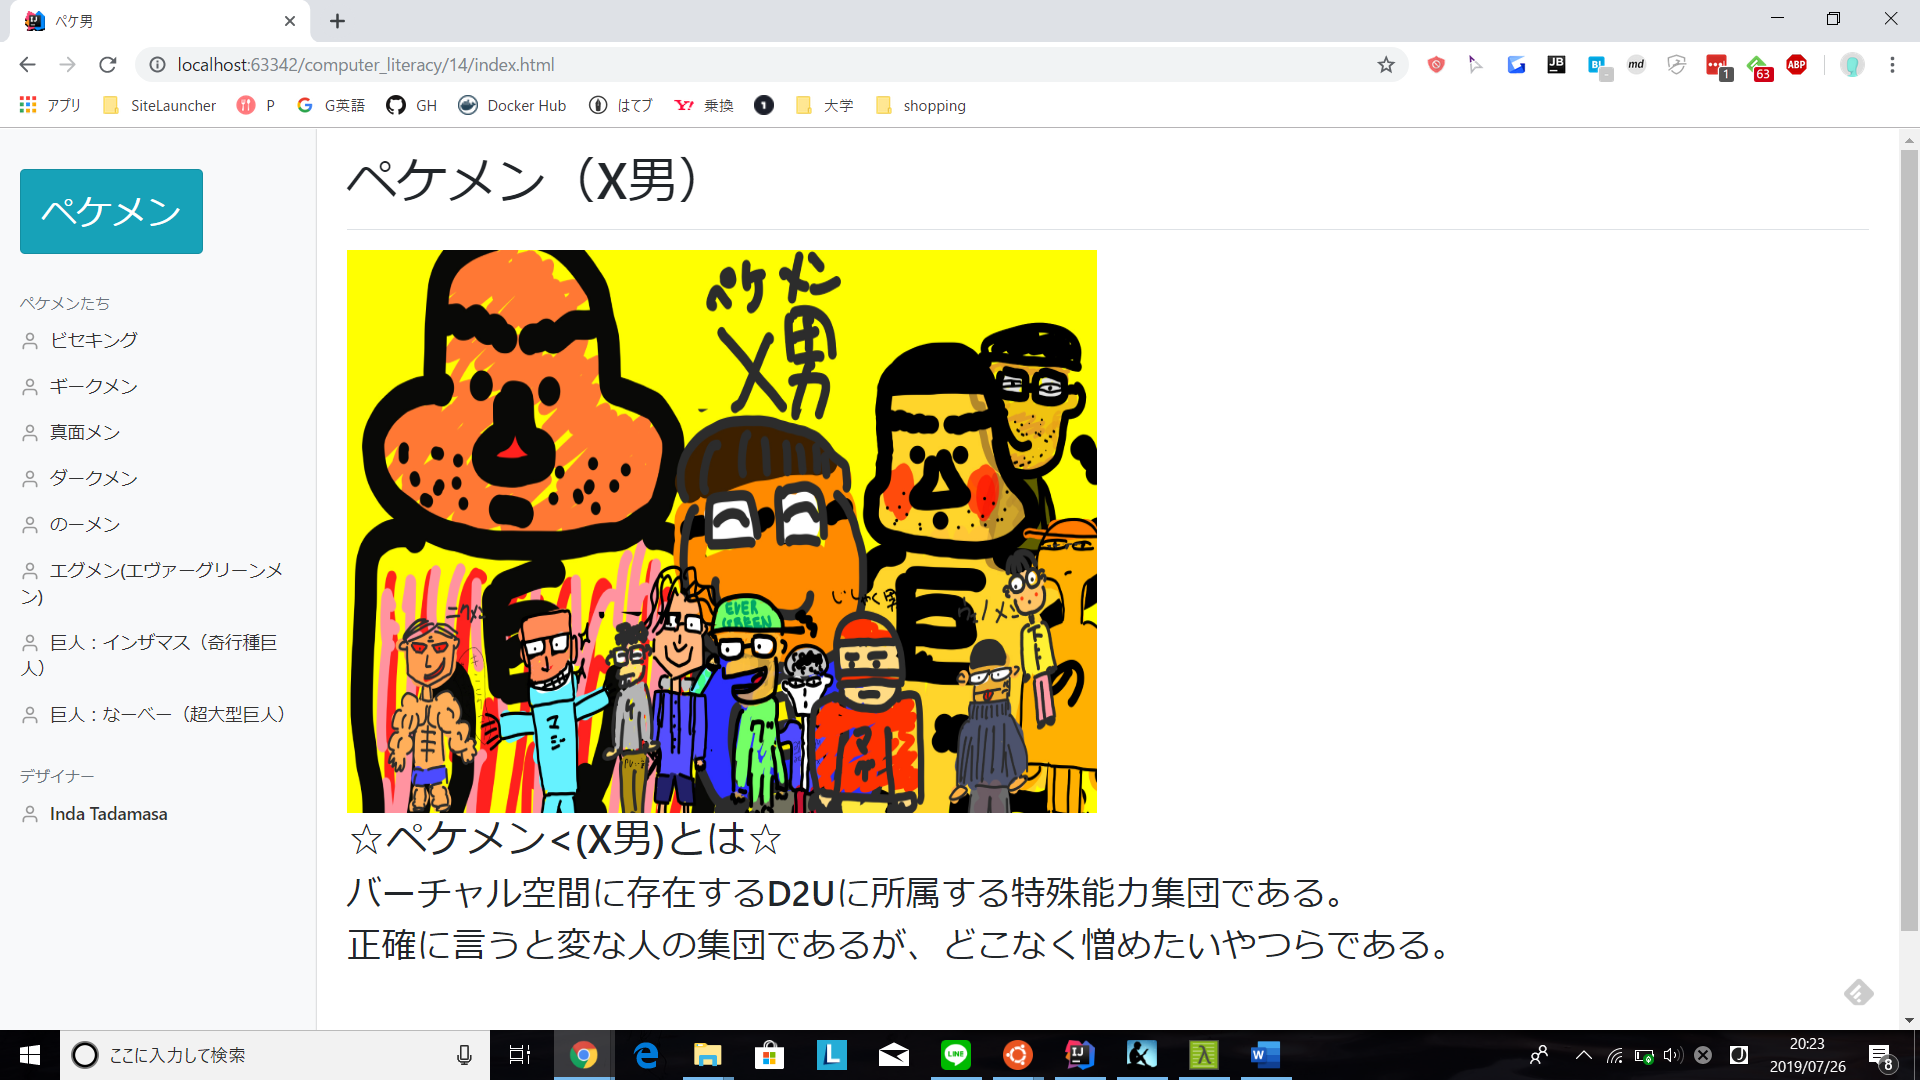
\includegraphics[width=10cm]{./index.png}
\end{center}

\subsubsection{各ヒーローのページ}

\begin{center}
  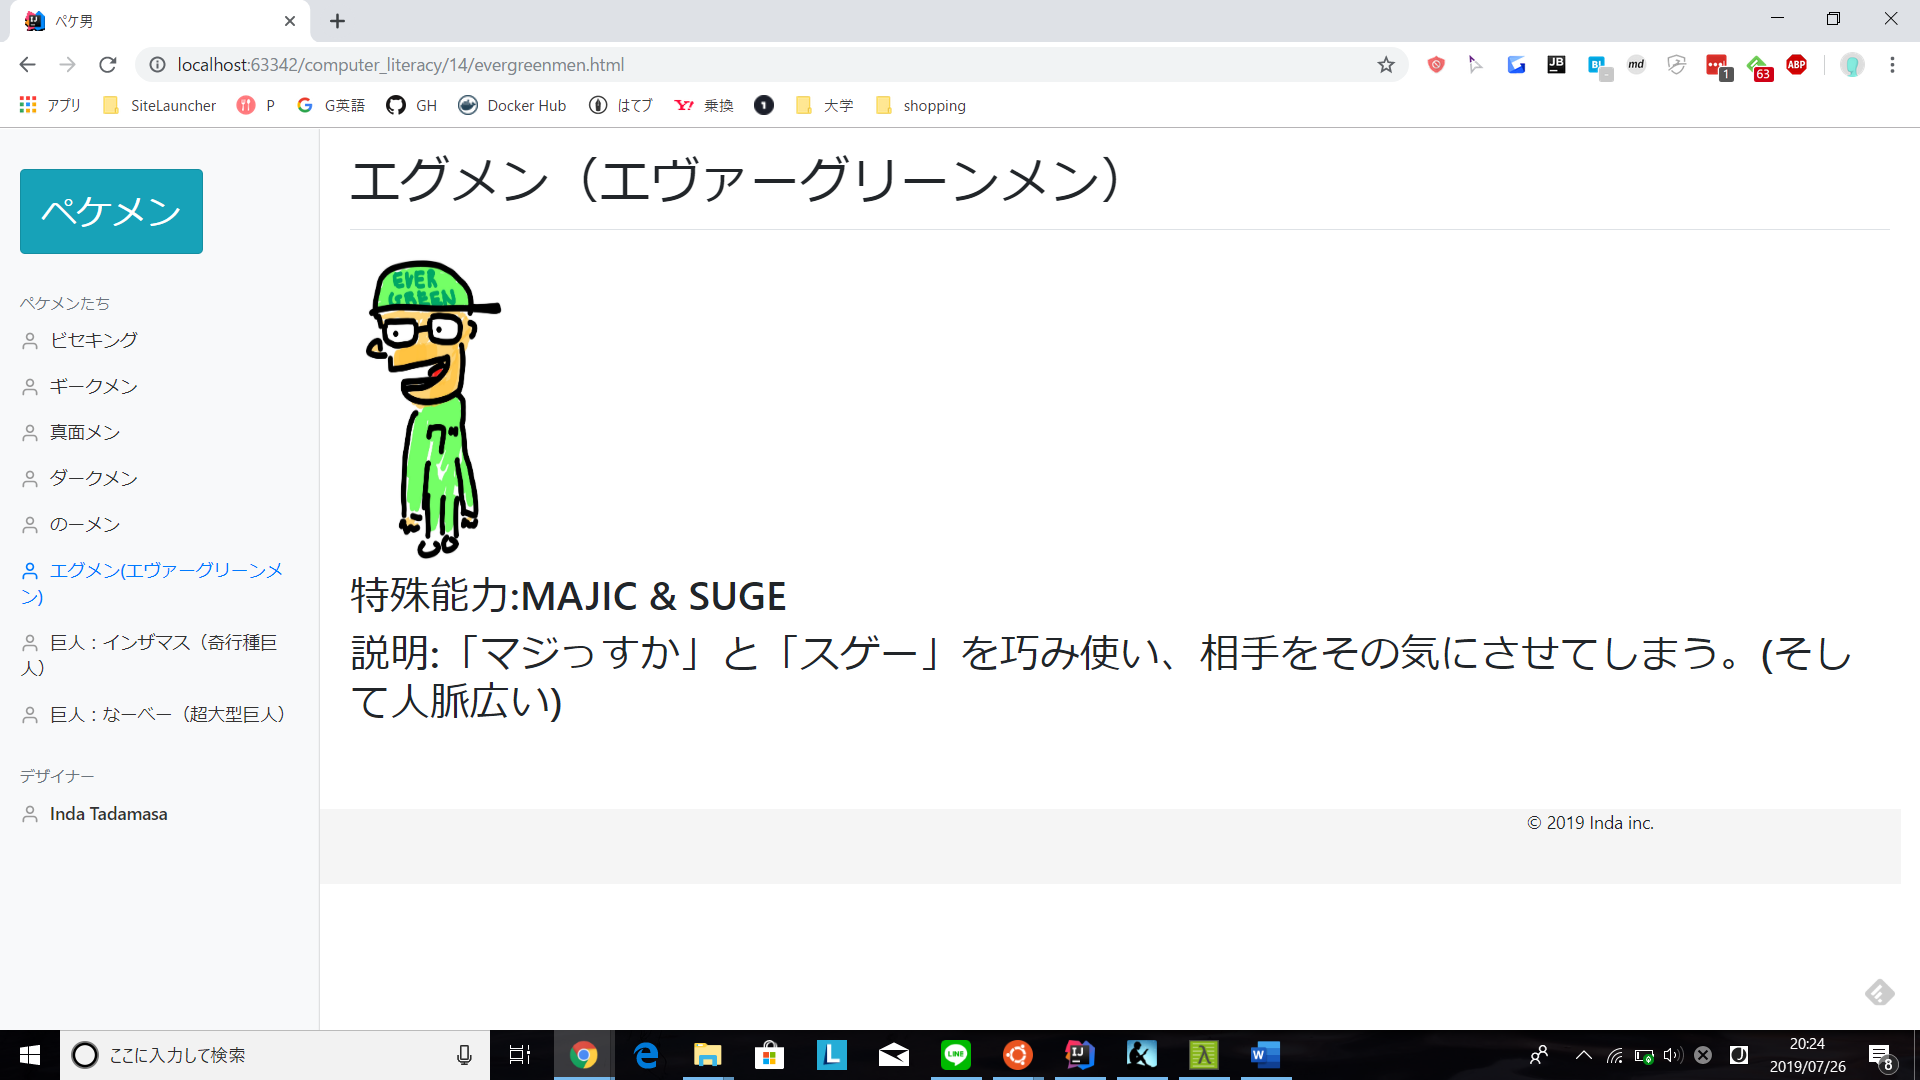
\includegraphics[width=10cm]{./hero1.png}
\end{center}

他の各ヒーローは共通のレイアウトなので省略する。

\subsubsection{ヒーローのデザイナーのページ}

\begin{center}
  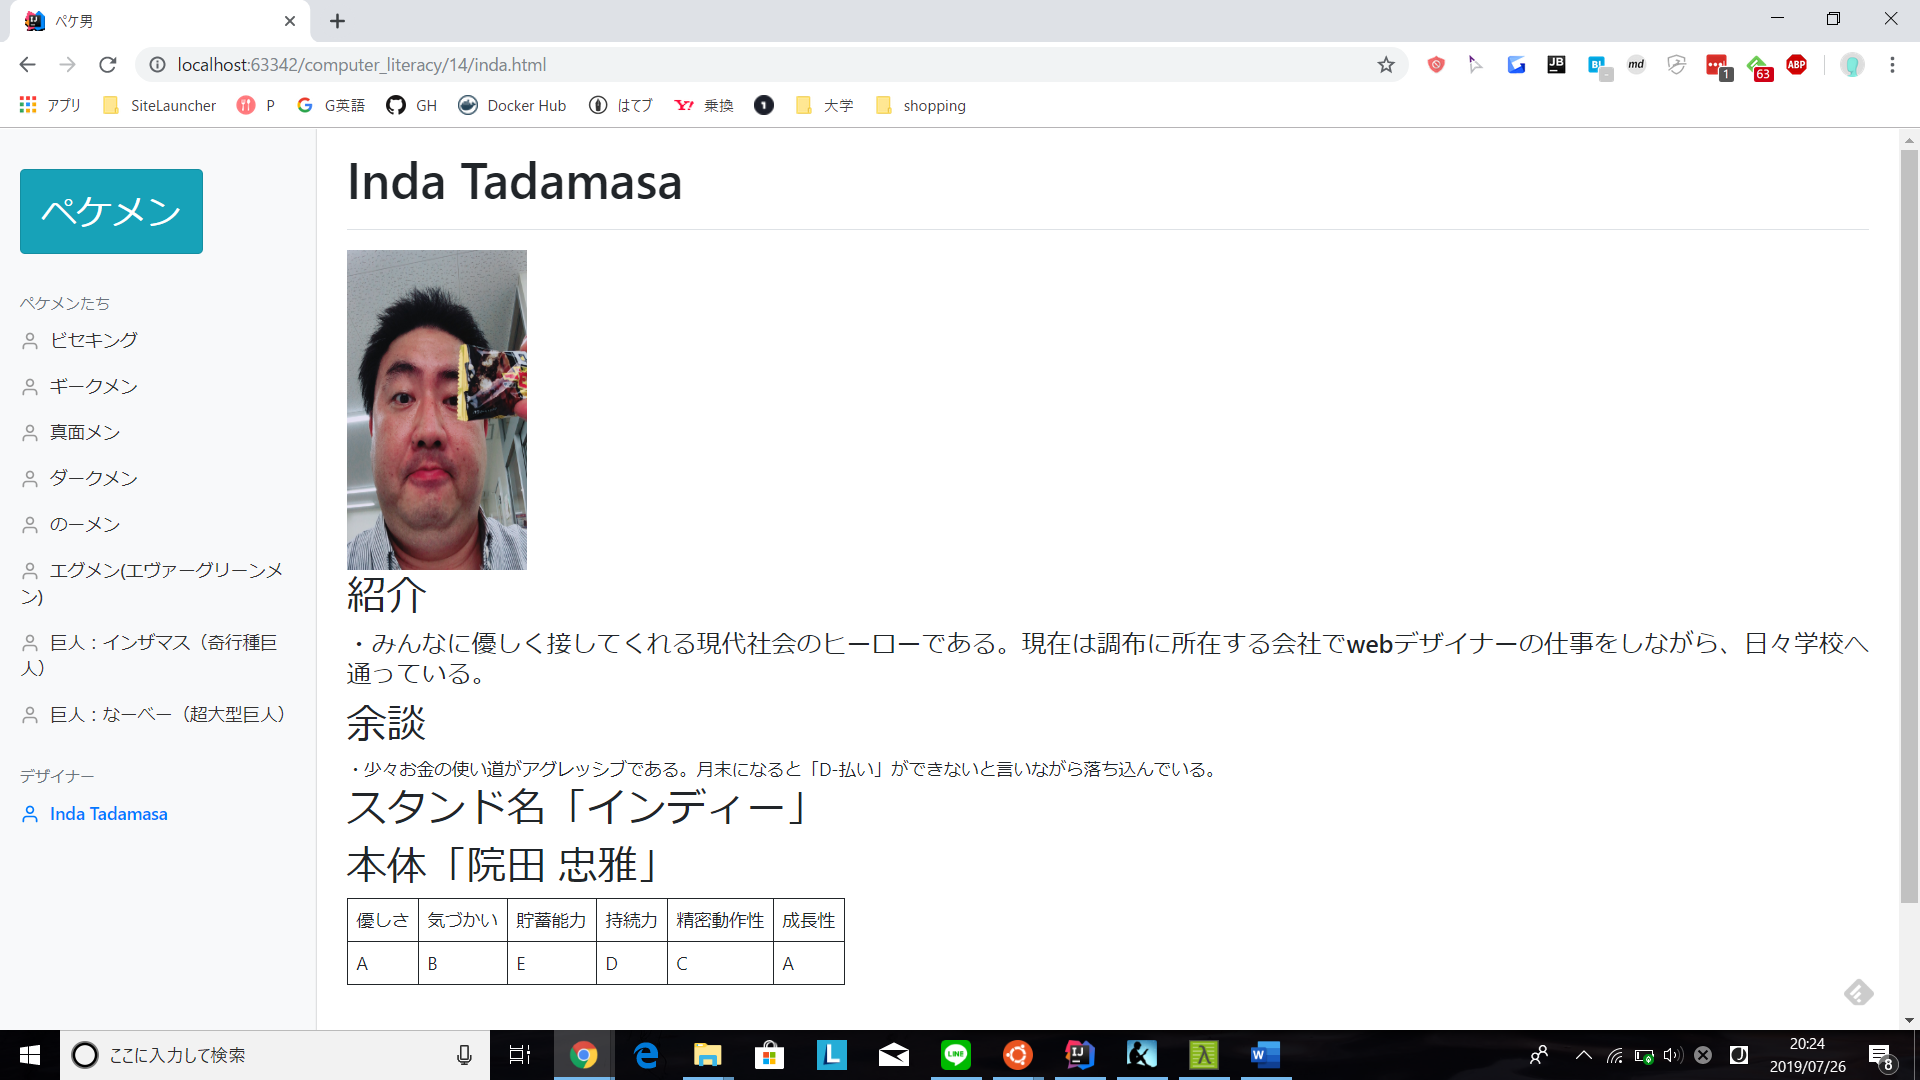
\includegraphics[width=10cm]{./designer.png}
\end{center}

%\begin{center}\includegraphics[width=10cm]{fig1.eps}\end{center}
% PostScriptの絵を入れたければ上の行の「%」をはずしファイル名を修正

\section{考察}

ファイル構造だが、普通なら複数改装にすべきだが、今回はグループワークであり作業を他人に割り振る必要がある。そのため、どこがどのディレクトリにあるのかお互いに連絡する必要があるのだが、それを省くために、すべてのファイルを同一に設置した。結果として、これのおかげで、ひな型のテンプレートを先に用意すれば特に何も言わなくても画像ファイルの用意や新しいファイルが作成されており戦略的には正解と判断できる。

今回は作業スピードを考慮して、私がトップページと各ヒーローページのテンプレートを作成して、内容を他のメンバーが入れ込む形にした。<h2>などの見出しタグさえ用意しておけば、各自適当なタグで説明文を書いてくれると予想していたが、<h2>タグに説明文を書いてしまったため、見出しと説明文でタグを分けられていなかった。のちに意図を理解してくれたメンバーが説明文を<p>タグなどの他のタグに切り出してくれて、タグの切り分けができた。今後チームでホームページを作成するときは、意図が伝わるように空のタグを用意しておいたほうが良い。

今回Bootstrap4を導入したが、フォントのサイズや色で余計にもめることがなく結果的に時間の節約は果たせた。CSSは最低限のみ書くようにした。CSSは、どこの部分のCSSかわかるように「サイドバー」「フッター」などのコメントを入れて、ファイルの中身を参照しただけで、どこの部分のCSSか理解できるように工夫した。結果として、このCSSはどこのCSSかということを聞かれることは1回もなかった。

画像についてだが、トップページのトップ画像だが、widthやheightをもと画像のまま出力すると全体のレイアウトが崩れてしまうので多少の画像比率の崩れを無視して縮小することになった。これにより画像によるページの崩れを防止した。

\section{参考文献}

Bootstrap4のサンプルサイト、これの「ダッシュボード」をカスタマイズして、作成した。

https://cccabinet.jpn.org/bootstrap4/example

テーブルの使用方法

https://www.kanzaki.com/docs/html/htminfo16.html

\section{アンケート}

\subsection{Q1:Webサイトをグループで協力して製作してみて、どのようなことが分かりましたか。}
グループワークなので、お互いに役割を決めて協力してやることが大事だと思いました。

\subsection{Q2:今回のようなレポートは何がよかったですか。何が大変でしたか。}
チームで協力するということは、他の人に何をどのようにしてほしいのか伝えなくてはならないため、齟齬の内容に伝えるのは大変でした。

\subsection{Q3:リフレクション (今回の課題で分かったこと)・感想・要望をどうぞ。}
ホームページを作成するのは、やはり結構大変だと思いました。だからホームページ作成サービスなどが存在するのかと思いました。



\end{document}v
